\chapter{DLC}

Úvod... schéma jednotlivých fází a typů dlc s vodíkem bez vodíku atd....

\section{Růst DLC vrstev}
Důležitým parametrem DLC vrstev je poměr sp3 a sp2 vázaného uhlíku. Experimentálně se ukázalo, že ideální postup pro dosažení nejvyššího poměru sp3 vazeb je iontové bombardování, přičemž nejvyšší sp3 koncentrace nastávají při depozicích ionty C$^+$ o energiích okolo 100\,eV. Následující popis depozičního mechanismu bude prvně proveden pro samotný uhlík (ta-C) a následně pro pro a-C:H.

Klíčovým faktem je to, že sp2 vázaný grafit má asi o 50\% větší objem než sp3 vázaný diamant. Z toho plyne, že pro větší tlaky dochází k fázové změně z sp2 na sp3. Princip depozice je tedy takový, že díky implantacím vysokoenergetických iontů pod povrch rostoucí vrstvy dochází k lokálnímu zhuštění materiálu a tím pádem přechodu od nejnižšího energetického stavu sp2 do sp3.

Podrobnější analýzou se ukazuje, že v pro energetickou oblast zájmu (cca 10--1000\,eV) je indentační hloubka iontů řádově jednotky nanometrů a ionty ztrácí energii především elastickými srážkami s atomy terče. Srážky můžeme aproximovat jako binární, takže celý proces zastavení iontu je potom řada nezávislých binárních srážek. Účinné průřezy pro srážku závisí na energii iontu a se stoupající energií klesají. Pro nízké energie, proto ion není schopen proniknout povrchem a skončí na povrchu rostoucí vrstvy v nejnižším energetickém stavu. Nejnižší energie, se kterou iont pronikne povrchem rostoucí vrstvy je $E_\mathrm{P}$ penetrační práh. 

Další důležitá energie je $E_\mathrm{d}$, je to minimální energie, kterou dopadající ion potřebuje k tmu, aby vyrazil navázaný atom vrstvy a vytvořil pár vakance -- intersticiál. Povrch se navíc chová jako přitažlivá potenciální bariéra o povrchové energii $E_\mathrm{B}$. O tuto energii se navýší energie iontu v momentě, kdy prochází povrchem. Celková energie potřebná pro iont k implantaci do vrstvy je proto $E_\mathrm{P} \sim E_\mathrm{d} - E_\mathrm{B}$. 

Pokud má tedy iont energii větší než $E_\mathrm{P}$, může proniknout do vrstvy a skončit jako intersticiál. Toho vede k lokálnímu zvýšení hustoty a k přeuspořádání lokálních vazeb podle nové hustoty. Jedná se o amorfní materiál, takže se nadá rozlišit mezi dopadajícím atomem a atomy původní mřížky. Se zvyšováním energie iontového bombardování se proto zvyšuje hustota materiálu a tím pádem se zvyšuje i množství sp3 vázaného uhlíku.

Část energie iontu se ztratí při průchodu povrchem, asi 30\% připadá na posuvy atomů původní mřížky [FIXME nějaká citace], zbytek se uvolní jako teplo. Právě nadměrné zahřívání umožňuje relaxaci vrstvy a je důvodem, proč klesá poměr sp3 vázaných atomů pro vysoké energie dopadajících iontů. Uvažujme dopadající svazek částic, z nichž je $\Phi$ energetických iontů s energií $E_\mathrm{i}$. Část $f$ dopadajících energetických iontů pronikne povrchem a implantuje se do vrstvy. Zbytek $(1-f \Phi)$, jedná se o ionty s nízkou energií a neutrální atomy, zůstane na povrchu vrstvy. U některých implantovaných iontů ale dojde k relaxaci zpět na povrch vrstvy. Toto záleží na tom, jaký je ve vrstvě poměr intersticiálů $n$. V rovnovážném stavu proto platí, že část iontů, která zůstane implantována jako intersticiály a přispívá ke zvyšování hustoty vrstvy je 
\begin{equation}
n = f \Phi - \beta n \text{,}
\end{equation}
kde $\beta$ je konstanta. Po úpravě dostáváme
\begin{equation}
n = \frac{f \Phi}{1 + \beta} \text{.}
\end{equation} 
Část $n$ původního svazku proto zůstane implantovaná ve vrstvě a část $1-n$ skončí na povrchu jako v sp2 hybridizaci. toto vede de zvýšení hustoty
\begin{equation}
\frac{\Delta \rho}{\rho} = \frac{n}{1-n} \text{,}
\end{equation}  
po dosazení
\begin{equation}
\frac{\Delta \rho}{\rho} = \frac{f \Phi}{1 - f \Phi + \beta} \text{,}
\end{equation}
kde $\rho$ je hustota sp2 uhlíku, $\Delta \rho$ je navýšení hustoty. Celý proces je schematicky znázorněn na obrázku \ref{dlcgrowth}.

\begin{figure}[htbp]
  \centering
  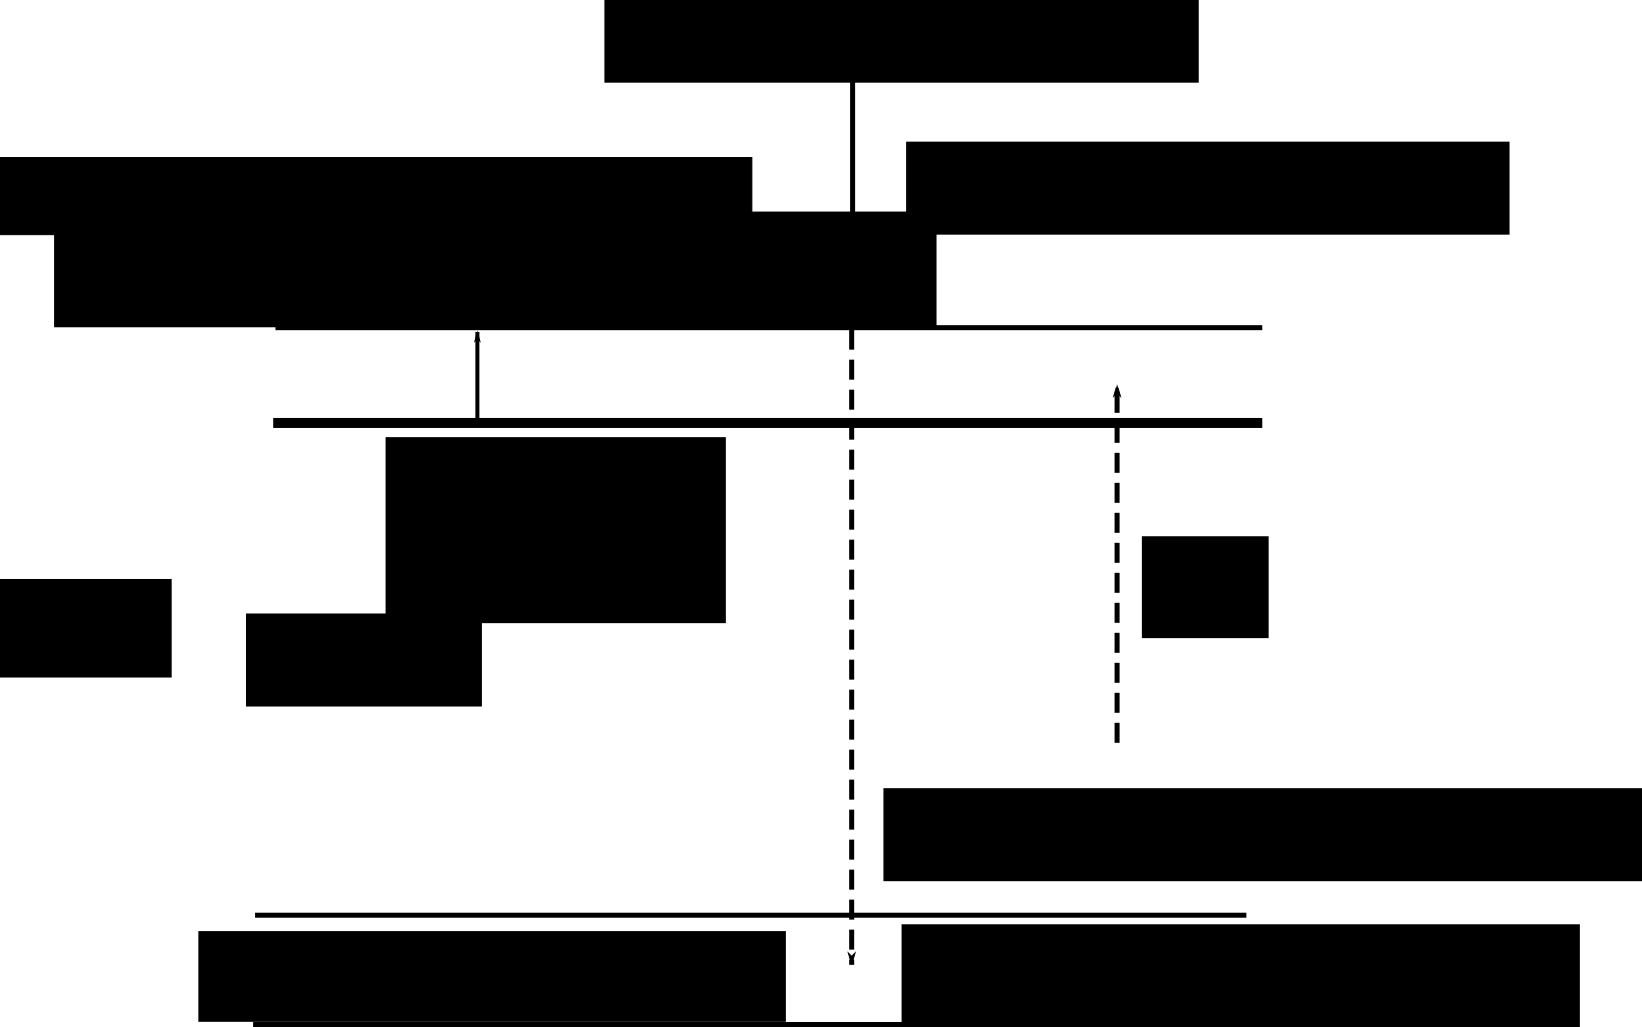
\includegraphics[width=100mm]{grafika/dlcgrowth.pdf}
  \caption{Schématický nákres růstu DLC vrstvy implantací energetických iontů, převzato z \cite{Robertson2002}.}
  \label{dlcgrowth}
\end{figure}

Implantace může navíc probíhat dvěma způsoby, buď přímou implantací dopadajícího atomu, případně srážkou dopadajícího atomu s atomem povrchu a implantací povrchového atomu do vrstvy (dopadající atom se odrazí). V případě molekulárního iontu (například acetylenu) dojde při srážce s povrchem s disociaci molekuly a implantaci každého atomu samostatně, přičemž kinetická energie se mezi ně rozdělí rovnoměrně \cite{Robertson2002}.

FIXME:víc citací

\section{Růst DLC vrstev s vodíkem}
Růst DLC vrstev s vodíkem je poněkud složitější než růst čistě uhlíkových vrstev. Podobně jako u čistě uhlíkových vrstev je i zde silná závislost na urychlovacím napětí a z toho plyne, že klíčovou úlohu opět hrají ionty. U depozic uhlovodíkových vrstev bývá tok iontů $Phi$ mnohem menší než u celouhlíkových vrstev, typicky kolem 10\% [nějaká citace], zbytek tvoří neutrální molekuly a atomy. Pro depozice uhlovodíkových vrstev je typický posuv maxima tvrdosti (tedy sp3 části) v závislosti na energii iontu v závislosti na depozičním plynu, konkrétně na jeho molekulové hmotnosti. 
Celková molekulová hmotnost je důležitá proto, že vlastnosti výsledné vrstvy závisí hlavně na energii dopadu v přepočtu na jeden atom a tak například benzenový iont C$_6$H$_6^+$ potřebuje přibližně šestkrát vyšší napětí pro urychlení než iont methanu CH$_3^+$. Při nárazu na povrch vrstvy dochází k disociaci molekuly a rozdělení energie mezi jednotlivé atomy podle zákona zachování hybnosti. Každý atom se potom implantuje samostatně. Některé další reakce při růstu vrstvy shrnuje obrázek \ref{dlcgrowthH}. Kromě C$_x$H$_y$ iontů jsou mezi dopadajícími částicemi i H atomy a ionty, C$_x$H$_y$ radikály a neutrální molekuly.

Povrch rostoucí vrstvy je plně pasivován C--H vazbami, dopadající monoradikály se proto můžou navázat pouze na povrchové volné vazby. Radikály se dvěma volnými vazbami se mohou vložit do existující C--C nebo C--H vazby. Pro neutrální molekuly jako CH$_4$a H$_2$ k žádným reakcím s vrstvou nedochází. Volné vazby na povrchu jsou vytvářeny buď vyražením atomárního vodíku při nárazu iontu a nebo reakcí s atomárním vodíkem a vznikem H$_2$ molekuly [nějaká další citace (Robertson 144)]. Atomy a atomární ionty vodíku také mohou kvůli své velikosti pronikat do vrstvy a způsobovat reakce ve vrstvě. Opět může docházet ke vznik molekulárního vodíku a volné vazby případně k repasivaci již existující volných vazech. Dopadající vodíkové ionty také způsobují leptání vrstvy a zpomalují rychlost růstu.

\begin{figure}[htbp]
  \centering
  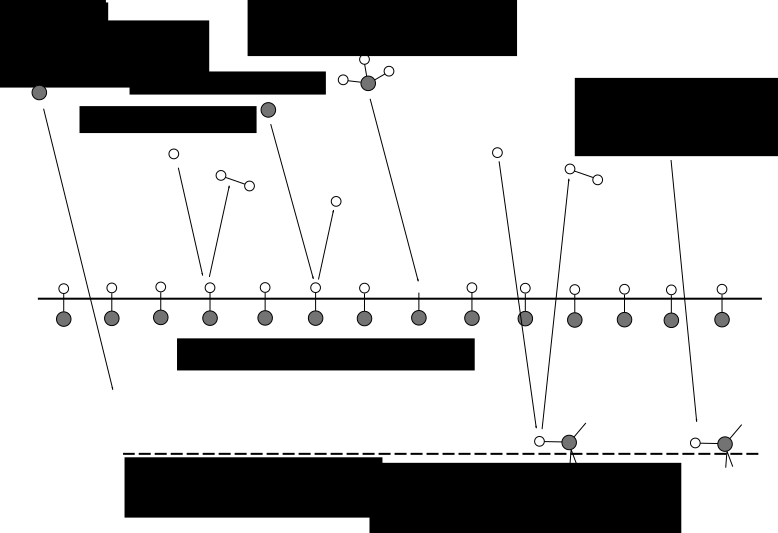
\includegraphics[width=150mm]{grafika/dlcgrowthH.pdf}
  \caption{Schématický nákres procesů růstu DLC vrstev s vodíkem, převzato z \cite{Robertson2002}.}
  \label{dlcgrowthH}
\end{figure}

Mezi klíčové parametry depozice patří vhodné zvolení depozičního plynu. Běžně používané plyny pro depozice DLC vrstev jsou jednoduché uhlovodíkové sloučeniny jako alkany (např. methan, ethan, propan, butan ...), alkeny (např. ethen), alkyny (např. acetylen), aromatické uhlovodíky (benzen) a další. Důležité parametry použitého plynu jsou ionizační energie, molekulární hmotnost a poměr vodíku k uhlíku. Pro nižší ionizační energie se rychlost depozice zvětšuje přibližně exponenciálně \cite{Koidl1991}. Z poměru uhlíku a vodíku se pak odvíjí poměr uhlíku a vodíku ve výsledné vrstvě a molekulární hmotnost určuje potřebné předpětí.

Pro depozici tvrdých ochranných vrstev se nejčastěji používá acetylen (C$_2$H$_2$), protože má po metanu nejnižší molekulovou hmotnost, nízkou ionizační energii, nízký obsah vodíku a sníženou míru plazmové polymerizace. Nevýhoda je, že není dostupný v čisté formě a obsahuje nějaké nečistoty jako například dusík \cite{Conway2000}. Z toho důvodu je pro depozici vrstev určených k optické charakterizaci nevhodný. Pro výrobu vrstev byl proto zvolen metan, který má sice vysokou ionizační energii (cca 12,4\,V), ale neobsahuje příměsi a kvůli jeho nízké molekulární hmotnosti není potřeba příliš velké předpětí při depozici.

FIXME: víc citací

\section{Kapacitně vázaný vysokofrekvenční doutnavý výboj}
\label{ccp}

Jedná se o jeden z nejvíce používaných typů nízkotlakých výbojů pro depozici DLC vrstev, je udržován vysokofrekvenčním rf proudem a napětím a je indukován přes kapacitní stěnovou vrstvu. V nejjednodušším uspořádání jsou nad sebou umístěny dvě elektrody. Na jednu z nich je přivedeno střídavé napětí, druhá je uzemněná, celý obvod navíc obsahuje blokovací kondenzátor. Schéma typického reaktoru je na obrázku \ref{reaktor-schema}. Rf výboj je pro PECVD výhodný jednak proto, že nedochází k nabíjení rostoucích dielektrických vrstev a je poměrně lehké dosáhnout vysokých urychlujících napětí. Urychlující napětí je zapříčiněno několika faktory. Základní jev je vznik stěnové vrstvy mezi plazmatem a elektrodami (a také stěnami rektoru). 
Elektrony totiž mají výrazně vyšší pohyblivost než ionty, proto je tok elektronů na stěny a elektrody řádově vyšší a dojde k jejich nabití záporným nábojem. K tomu jsou přitahovány kladné ionty z plazmatu a elektrony jsou naopak odpuzovány,až dojde ke kompenzaci toku elektronů i iontů způsobených rozdílnou pohyblivostí. Mezi plazmou a povrchem tak vzniká oblast ve které je rozdílná koncentrace iontů a elektronů a potenciál v ní klesá od potenciálu plazmatu na potenciál povrchu. Nejedná se už o plazma, protože to je z definice kvazineutrální. 
Vznik stěnové vrstvy je typický pro jakékoli plazma a neomezuje se na vysokofrekvenční výboj. Další zvýšení předpětí ve stěnové vrstvě ze způsobeno aplikací střídavého napětí. Během kladné fáze kopíruje plazmový potenciál aplikované napětí, během záporné fáze se ale plazmový potenciál řídí nejvyšším napětím v systém, v tomto případě nulovým napětím uzemněné elektrody. Protože ionty mají malou pohyblivost a nestíhají kopírovat aktuální výchylky potenciálu, ale jen jejich střední hodnoty, dochází k navýšení celkového potenciálu v plazmatu a tím i předpětí ve stěnové vrstvě.  
Poslední faktor, který vede ke zvýšení předpětí je rozdílná velikost elektrod, která vede k tomu, že předpětí je větší na menší elektrodu \cite{liebermandischarge, chen2003sheet}
\begin{equation}
\frac{U_1}{U_2} = \left(\frac{A_2}{A_1}\right)^2 \text{,}
\end{equation}
kde $A_1$, $A_2$ jsou plochy elektrod a $U_1$, $U_2$ jsou napětí na elektrodách.

FIXME: tohle asi ještě rozepsat víc (srážky ve stěnové vrstvě, polymerizace, vyhasínání při nízkých tlacích atd...)

\begin{figure}[htbp]
  \centering
  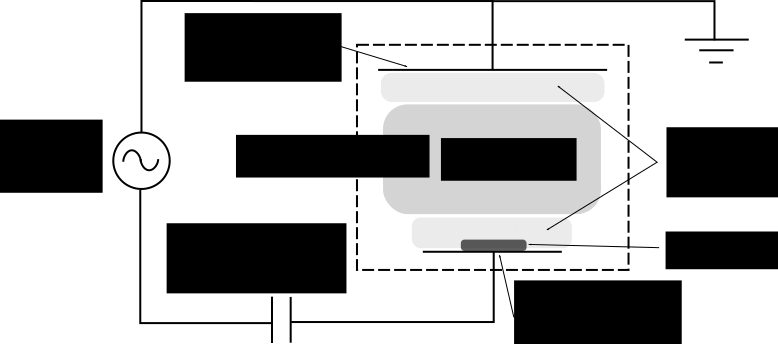
\includegraphics[width=120mm]{grafika/reaktor.pdf}
  \caption{Schéma reaktoru pro vysokofrekvenční kapacitně vázaný výboj}
  \label{reaktor-schema}
\end{figure}

\cleardoublepage
